
%(BEGIN_QUESTION)
% Copyright 2012, Tony R. Kuphaldt, released under the Creative Commons Attribution License (v 1.0)
% This means you may do almost anything with this work of mine, so long as you give me proper credit

This elevator control system has a problem.  No matter which pushbutton is pressed, the elevator remains ``stuck'' in the full-down position.  The following pictorial diagram shows the wiring of this system, along with the I/O card status lights as they appear with no one pressing any pushbuttons:

$$\includegraphics[width=15.5cm]{i02538x01.eps}$$

Pressing the ``Down'' and ``Up'' pushbuttons, you notice the LEDs for input channels 0 and 3 light up, respectively.  No LEDs on the output card light up at any time.

\vskip 10pt

Based on this information, determine a likely fault causing this elevator to remain stuck at the full-down position.

\underbar{file i02538}
%(END_QUESTION)





%(BEGIN_ANSWER)

The ``Up'' limit switch is failed shorted, making the PLC ``think'' the elevator is in the full-up position, which prevents it from trying to move upwards.  The elevator will not move down either, because the ``Down'' limit switch properly indicates the platform's full-down position, preventing any further downward motion.

\vskip 10pt

We may tell this is the fault by examining the LED status indicators on the input card for the two limit switches.  You will note that both channels 1 and 2 are lit, indicating {\it both} limit switches are sending signals to the PLC's input card.  According to the symbols shown on the limit switches themselves, these are normally-open (NO) switches, which means they should pass power to the PLC only if they detect the presence of the elevator platform.  When the platform is not at one of those positions, the switch is supposed to return to its resting state (open) and thereby de-energize its respective PLC input channel.

The fact that both LEDs are lit is an indication something is wrong with the limit switches.  Seeing that both limit switches have NO contacts, and knowing the elevator platform happens to be in the fully down position, we may conclude that the ``up'' limit switch is failed shorted.

%(END_ANSWER)





%(BEGIN_NOTES)


%INDEX% PLC, troubleshooting: elevator control system

%(END_NOTES)


